\documentclass[sn-mathphys-num]{sn-jnl}
\usepackage{graphicx}
\usepackage{multirow}
\usepackage{amsmath,amssymb,amsfonts}
\usepackage{amsthm}
\usepackage{booktabs}
\newtheorem{lemma}{Lemma}
\newtheorem{proposition}{Proposition}
\raggedbottom
\setlength{\textfloatsep}{5pt plus 2pt minus 2pt}
\setlength{\intextsep}{4pt plus 2pt minus 2pt}
\setlength{\floatsep}{4pt plus 2pt minus 2pt}
\setlength{\abovecaptionskip}{3pt}
\setlength{\belowcaptionskip}{1pt}
\setlength{\parskip}{0pt}
\let\OLDthebibliography\thebibliography
\renewcommand\thebibliography[1]{\OLDthebibliography{#1}\setlength{\itemsep}{0pt}\setlength{\parskip}{0pt}\setlength{\parsep}{0pt}\clubpenalty=10000\widowpenalty=10000\interlinepenalty=100}
\makeatletter
\renewcommand\section{\@startsection{section}{1}{\z@}{-10pt \@plus -3pt \@minus -2pt}{6pt}{\sectionfont}}
\renewcommand\subsection{\@startsection{subsection}{2}{\z@}{-9pt \@plus -3pt \@minus -2pt}{4pt}{\subsectionfont}}
\renewcommand\paragraph{\@startsection{paragraph}{4}{\z@}{-9pt \@plus -3pt \@minus-1pt}{2pt}{\paragraphfont}}
\makeatother

\raggedbottom
\begin{document}

\title[Behavioural trigger probing for federated backdoors]{Score Quality Versus Decision Quality: Why Behavioural Trigger Probing for Federated Backdoors Fails Under Heterogeneity, and When a Different Decision Rule Recovers It}

\author*[1]{\fnm{Mihit} \sur{Nanda}}\email{mihitnanda2005@gmail.com}

\affil*[1]{\orgdiv{Department of Computer Science and Engineering}, \orgname{IILM University}, \orgaddress{\city{Greater Noida}, \state{Uttar Pradesh}, \country{India}}}

\abstract{Backdoor attacks on federated learning (FL) implant a hidden trigger--target behaviour through a minority of poisoned clients. Behavioural (model-inspection) defences probe candidate client models with trigger patches rather than inspecting update geometry. This paper's thesis is narrower than proposing a new detector: \emph{behavioural probing carries information about backdoors, but statistical heterogeneity can create a mismatch between how separable that information is (score quality) and whether a fixed decision rule extracts it (decision quality)}. Using \textbf{ProbeGuard} (a flip-rate behavioural score) as the vehicle, we show late-round AUROC stays $\ge0.95$ for $\alpha\ge0.5$ while a fixed MAD threshold nonetheless collapses under heterogeneity (TPR 0.0 at $\alpha{=}0.1$ vs.\ 0.94 at $\alpha{=}10$); we trace this mechanistically to benign score spread, which shrinks monotonically with heterogeneity and correlates with the collapse ($r=-0.82$). A decision-rule sweep (percentile thresholds, a rank-based rule, an oracle ceiling) shows the fixed-threshold family is the problem, not the representation: a rank-based rule tracks the oracle closely for $\alpha\ge0.5$. We test this rank-based rule on unseen seeds, under a probe-aware adaptive attacker that optimises against the score directly, and in a compute-constrained CNN/CIFAR-10 stress test -- it remains comparatively robust in all three, though the adaptive attacker narrows the gap under heterogeneity and the CNN stress test shows the underlying failure mode does not shrink at larger scale. Negative and unresolved results (an ineffective scoring-rule ablation, an unexplained FLTrust collapse on CNNs) are reported as such, not hidden.}

\keywords{federated learning, backdoor attacks, model inspection, non-IID heterogeneity, robust aggregation, trustworthy machine learning}

\maketitle

\section{Introduction}\label{sec1}
Federated learning trains a shared model without centralising raw data~\cite{mcmahan2017fedavg}, but the openness of the training protocol lets a minority of clients implant backdoors: behaviours that are dormant on clean inputs and triggered by an attacker-chosen pattern~\cite{gu2019badnets,bagdasaryan2020backdoor,bhagoji2019adversarial}. Defences broadly operate on update \emph{geometry} (distance-based selection, medians, clipping)~\cite{blanchard2017krum,yin2018byzantine,sun2019really}, on trust anchored by a server dataset~\cite{cao2021fltrust}, or on model \emph{inspection}~\cite{rieger2022deepsight,nguyen2022flame}. Outside FL, backdoor detectors probe a model's behaviour with candidate triggers~\cite{wang2019neuralcleanse,kolouri2020ulp}.

A persistent difficulty in FL is statistical heterogeneity: with non-IID clients, benign updates are themselves dispersed~\cite{hsu2019measuring,li2020fedprox}, blurring the line between benign and malicious. Defence papers commonly report a single heterogeneity level, and commonly conflate ``the score is uninformative'' with ``the chosen threshold on that score fails.'' This paper keeps those separate: \emph{for a behavioural backdoor detector, does detection degrade because the underlying signal vanishes, or because a fixed decision rule is the wrong tool for a signal whose benign spread changes with heterogeneity -- and if the latter, does any practical decision rule do better?}

\paragraph{Contributions.}
(i) We separate \emph{score quality} (AUROC/AUPRC) from \emph{decision quality} (realised TPR/FPR/ASR) across heterogeneity and show they diverge (Section~\ref{sec6}). (ii) A mechanism: a median-containment lemma (Section~\ref{sec4}) plus a measured link from heterogeneity to benign score spread to MAD-rule failure. (iii) A six-way decision-rule sweep (MAD, three percentiles, rank-based, oracle ceiling) on the same score. (iv) Root-set/probe-bank ablations, unknown-$f$ misspecification, and computational overhead. (v) We test a probe-aware adaptive attacker that optimises directly against the score, and report an ASR-over-rounds analysis and a CNN/CIFAR-10 stress test. (vi) We report negative and unresolved results as such: percentile rules do not fix the MAD rule's failure, an FLTrust collapse on CNNs is flagged unresolved rather than explained away, and we do not claim state-of-the-art, adversarially-optimal, or trigger-family-general robustness beyond what was tested.

\section{Related work}\label{sec2}
\textbf{Backdoors in FL.} Model-replacement/constrain-and-scale attacks~\cite{bagdasaryan2020backdoor}, adversarial-lens analyses~\cite{bhagoji2019adversarial}, distributed triggers~\cite{xie2020dba} and edge-case backdoors~\cite{wang2020tails} show a small malicious fraction suffices. \textbf{Robust aggregation.} Krum/Multi-Krum~\cite{blanchard2017krum}, coordinate median/trimmed mean~\cite{yin2018byzantine}, and norm clipping~\cite{sun2019really} are standard; FLTrust bootstraps trust from a server root set~\cite{cao2021fltrust}; FoolsGold targets Sybil similarity~\cite{fung2020foolsgold}. \textbf{Model inspection.} DeepSight~\cite{rieger2022deepsight} and FLAME~\cite{nguyen2022flame} inspect model internals; Neural Cleanse~\cite{wang2019neuralcleanse} and Universal Litmus Patterns~\cite{kolouri2020ulp} probe with candidate/learned triggers outside FL. ProbeGuard is closest in spirit to the latter two; our contribution is the heterogeneity-stratified score-vs-decision-rule analysis, not a claim of a stronger detector.

\section{Problem setting}\label{sec3}
$n$ clients hold local datasets; $\mathcal{M}$ ($|\mathcal{M}|=m<n/2$) is malicious. In round $t$, client $i$ returns update $u_i$ from server model $w_t$. Malicious clients relabel a fraction $\rho$ of non-target samples after stamping trigger $\tau$. The server holds a small clean root set $D_0$ (also used by FLTrust) and applies $w_{t+1}=w_t+\mathrm{Agg}(u_1,\dots,u_n)$. Goal: low attack success rate (ASR, fraction of triggered non-target test inputs classified as target) at unchanged clean accuracy. Attackers are non-adaptive (the threat model above).

\section{Method: ProbeGuard}\label{sec4}
\begin{figure}[htbp]
\centering
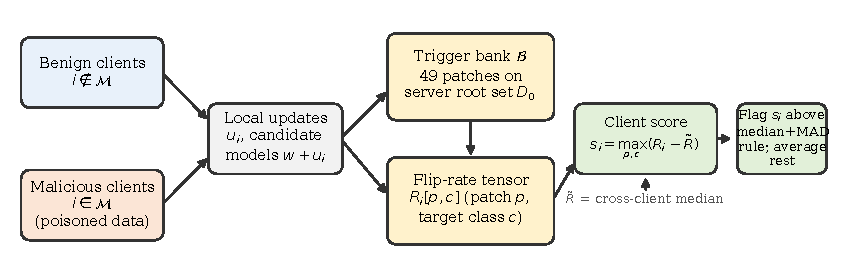
\includegraphics[width=0.7\textwidth]{fig_pipeline.pdf}
\caption{ProbeGuard per-round pipeline. Each candidate model $w+u_i$ is probed with a bank of patches on the server root set; the flip-rate tensor is compared with the cross-client median and clients with anomalous excess are excluded before averaging.}\label{fig:pipeline}
\end{figure}

\paragraph{Probe bank.} $\mathcal{B}$ is the set of all $2\times2$ saturated patches at the $49$ positions of an $8\times8$ image (ProbeGuard+ adds a second intensity, giving $98$). By construction the probe patch size equals the \textit{fixed}/\textit{multi}/\textit{lowint} trigger size ($2\times2$ digits, $4\times4$ CIFAR-10, same $H/8$ rule); the \textit{large} ($3\times3$) digits attack is deliberately unmatched to any probe cell, so detecting it (Section~\ref{sec6}) tests generalisation beyond exact probe geometry.
\paragraph{Threat model.} The attacker is assumed able to: poison local training data; control a minority of clients ($m<n/2$); know the target class and trigger used. The attacker is explicitly \emph{not} assumed to: know that ProbeGuard is deployed; optimise the poisoned update against the probe score; collude beyond shared poisoning; or manipulate model response to probes directly. Claims in this paper should be read against this threat model throughout.
\paragraph{Flip-rate tensor.} For candidate model $f_i=f(w+u_i)$ and cell $(p,c)$,
\[
R_i[p,c]=\frac{\#\{x\in D_0: y(x)\neq c,\ f_i(\mathrm{stamp}_p(x))=c\}}{\#\{x\in D_0: y(x)\neq c\}}.
\]
\paragraph{Score and decision.} With $\tilde R$ the cellwise median over clients, $s_i=\max_{p,c}(R_i[p,c]-\tilde R[p,c])$. The \emph{MAD rule} flags $i$ if $s_i>\operatorname{med}(s)+\max(k\cdot\mathrm{MAD}(s),\delta)$, and the server averages the unflagged updates (if all are flagged, none are). \emph{ProbeGuard-K} (post hoc, Section~\ref{sec6}) instead drops the $f$ highest scores, with $f$ assumed known exactly as for Multi-Krum.

\begin{lemma}[Median containment]\label{lem1}
If $m<n/2$, then for every cell $\min_{j\notin\mathcal{M}}R_j[p,c]\le\tilde R[p,c]\le\max_{j\notin\mathcal{M}}R_j[p,c]$.
\end{lemma}
\begin{proof}
Let $v$ be either middle order statistic of the $n$ values in a cell. At least $\lceil n/2\rceil>m$ values are $\le v$, so at least one benign value is $\le v$; likewise at least one benign value is $\ge v$. The median is $v$ or the mean of the two middle order statistics, hence lies between the smallest and largest benign values.
\end{proof}
\begin{proposition}[Score-level separability]\label{prop1}
Let $\Delta_B=\max_{p,c}\big(\max_{j\notin\mathcal{M}}R_j[p,c]-\min_{j\notin\mathcal{M}}R_j[p,c]\big)$ be the benign spread. If $m<n/2$, every benign client has $s_j\le\Delta_B$, and a malicious client with trigger cell $(p^\ast,c^\ast)$ has $s_i\ge R_i[p^\ast,c^\ast]-\max_{j\notin\mathcal{M}}R_j[p^\ast,c^\ast]$. Hence all malicious scores exceed all benign scores whenever the trigger response exceeds the benign maximum in its cell by more than $\Delta_B$.
\end{proposition}
\begin{proof}
By Lemma~\ref{lem1}, $R_j-\tilde R\le\max_B R-\min_B R\le\Delta_B$ for benign $j$, and $\tilde R\le\max_B R$ gives the malicious bound.
\end{proof}
The condition is sufficient, not necessary, but it identifies the mechanism: $\Delta_B$ measures how differently benign models respond to saturated patches. Heterogeneity increases $\Delta_B$ because class-skewed models flip towards their dominant classes; the empirical benign 95th-percentile score in Section~\ref{sec6} (1.00 at $\alpha{=}0.1$ down to 0.47 at $\alpha{=}10$) is consistent with this. The proposition concerns scores, not the thresholded rule, which additionally depends on $\mathrm{MAD}(s)$ and on early-round model state.

\section{Experimental setup}\label{sec5}
\paragraph{Data and model.} We use the scikit-learn digits dataset (1{,}797 images, $8\times8$)~\cite{pedregosa2011sklearn}, split per seed into 1{,}200 training, 100 server root and 497 test images. The model is a $64$--$32$--$10$ ReLU MLP trained with SGD (lr $0.1$, batch $32$, $2$ local epochs), implemented in NumPy~\cite{harris2020numpy}. There are $n=20$ clients, $30$ rounds, full participation, Dirichlet partitions with $\alpha\in\{0.1,0.5,1,10\}$.
\paragraph{Attacks.} Target class $0$; malicious clients (default $m=4$, 20\%) poison $50\%$ of their non-target samples with no update boosting. Triggers: \textit{fixed} ($2\times2$, intensity 1, bottom-right), \textit{multi} (one of four corners per sample), \textit{lowint} ($2\times2$, intensity 0.5) and \textit{large} ($3\times3$, intensity 0.75). ASR is computed on non-target test images stamped with the same trigger family.
\paragraph{Baselines.} FedAvg, coordinate median, 20\%-trimmed mean, norm clipping to the median norm, Multi-Krum (given the true $f$, an advantage), FLTrust (root update from 2 epochs on $D_0$), and a benign-only oracle. Baseline implementations are our own simplified versions.
\paragraph{Protocol.} $k$ and $\delta$ were tuned on validation seeds 100--102 at $\alpha{=}1$ (grid $k\in\{2,3.5,5\}$, $\delta\in\{0.1,0.2,0.3\}$), giving $k{=}2,\delta{=}0.1$. Test seeds are 0--7; ProbeGuard-K and a re-run of key baselines use unseen seeds 20--27. We report means with 95\% $t$-intervals, paired exact Wilcoxon tests~\cite{wilcoxon1945} and Holm correction~\cite{holm1979} within two pre-specified families (ProbeGuard versus FedAvg; versus the best baseline per $\alpha$, chosen post hoc on the same data, which is conservative against ProbeGuard).

\section{Results}\label{sec6}
\subsection{Heterogeneity dependence}
\begin{table}[htbp]
\caption{Fixed-trigger attack, 20\% malicious clients; mean $\pm$ 95\% CI over 8 seeds.}\label{tab:main}
\centering\footnotesize
\setlength{\tabcolsep}{3.5pt}\begin{tabular}{@{}lcccc@{}}
\toprule
Defence & $\alpha{=}0.1$ & $\alpha{=}0.5$ & $\alpha{=}1$ & $\alpha{=}10$\\
\midrule
\multicolumn{5}{@{}l}{\emph{Attack success rate (\%, lower is better)}}\\
FedAvg & 79.9$\pm$13.3 & 77.4$\pm$5.5 & 76.2$\pm$5.7 & 69.9$\pm$3.4\\
Coord. median & 16.6$\pm$7.8 & 5.3$\pm$4.0 & 3.4$\pm$3.3 & 0.7$\pm$0.5\\
Trimmed mean & 26.9$\pm$10.4 & 6.2$\pm$3.0 & 3.9$\pm$3.5 & 1.1$\pm$0.8\\
Norm clip & 82.4$\pm$11.0 & 76.5$\pm$5.0 & 67.5$\pm$8.8 & 36.3$\pm$10.6\\
Multi-Krum & 85.4$\pm$12.1 & 82.0$\pm$10.7 & 18.1$\pm$23.4 & 15.8$\pm$23.9\\
FLTrust & 24.0$\pm$14.1 & 5.3$\pm$7.2 & 2.6$\pm$3.5 & 0.3$\pm$0.3\\
ProbeGuard & 80.2$\pm$13.4 & 70.3$\pm$6.7 & 46.8$\pm$21.4 & 0.3$\pm$0.2\\
ProbeGuard+ & 80.2$\pm$13.4 & 70.3$\pm$6.7 & 43.4$\pm$20.0 & 0.3$\pm$0.2\\
Oracle (benign only) & 0.1$\pm$0.1 & 0.2$\pm$0.2 & 0.2$\pm$0.3 & 0.1$\pm$0.1\\
\midrule
\multicolumn{5}{@{}l}{\emph{Clean accuracy (\%, higher is better)}}\\
FedAvg & 80.4$\pm$3.6 & 88.1$\pm$1.5 & 88.3$\pm$1.6 & 88.2$\pm$1.4\\
Coord. median & 55.0$\pm$7.4 & 80.9$\pm$3.9 & 86.2$\pm$1.7 & 88.1$\pm$1.2\\
Trimmed mean & 60.1$\pm$7.4 & 84.6$\pm$2.5 & 87.4$\pm$1.7 & 88.1$\pm$1.4\\
Norm clip & 76.2$\pm$6.0 & 86.8$\pm$1.7 & 87.6$\pm$1.6 & 87.2$\pm$1.6\\
Multi-Krum & 67.7$\pm$8.2 & 84.0$\pm$3.9 & 88.7$\pm$1.7 & 89.1$\pm$1.2\\
FLTrust & 76.7$\pm$3.8 & 86.2$\pm$1.3 & 89.4$\pm$2.2 & 91.9$\pm$1.0\\
ProbeGuard & 80.2$\pm$3.4 & 87.9$\pm$1.7 & 88.8$\pm$1.6 & 89.2$\pm$1.5\\
ProbeGuard+ & 80.2$\pm$3.4 & 87.9$\pm$1.7 & 88.8$\pm$1.6 & 89.2$\pm$1.4\\
Oracle (benign only) & 81.4$\pm$3.2 & 88.4$\pm$0.7 & 89.2$\pm$1.8 & 89.3$\pm$1.1\\
\bottomrule
\end{tabular}
\end{table}
\begin{figure}[htbp]
\centering
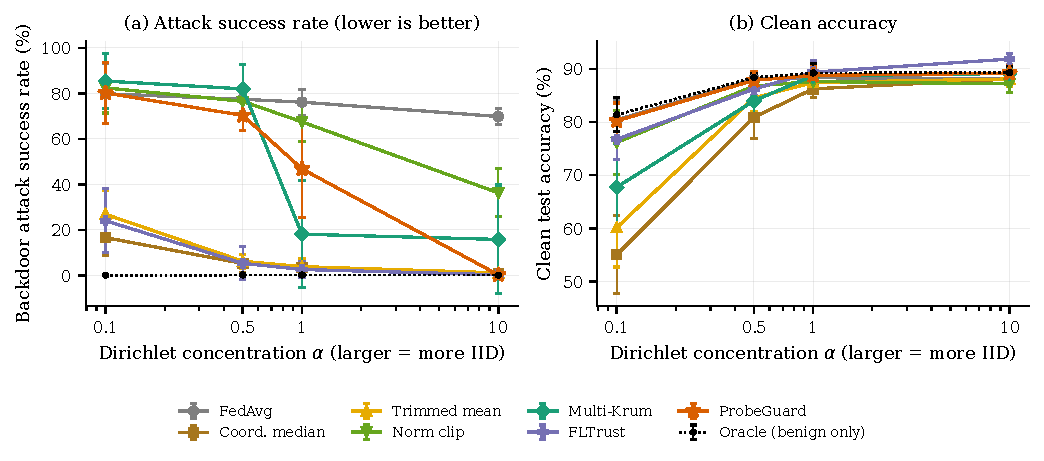
\includegraphics[width=0.82\textwidth]{fig_alpha.pdf}
\caption{Attack success rate and clean accuracy versus heterogeneity (fixed trigger, 20\% malicious). Error bars: 95\% CI over 8 seeds.}\label{fig:alpha}
\end{figure}
Table~\ref{tab:main} and Fig.~\ref{fig:alpha} show a sharp regime dependence. At $\alpha{=}10$, ProbeGuard attains 0.3\% ASR at 89.2\% clean accuracy (oracle 89.3\%), versus 69.9\% for FedAvg; no statistically significant difference from FLTrust was detected (paired $\Delta=-0.03$\,pp, $p=0.63$; Table~\ref{tab:stats}) -- this is not evidence of equivalence, only of an undetected difference at $n=8$. At $\alpha{=}1$ ASR rises to 46.8\% with a wide interval, and at $\alpha\le0.5$ ProbeGuard is not meaningfully better than FedAvg (70.3\% at $\alpha{=}0.5$; the $-7.1$\,pp difference is not significant after correction). Coordinate median and FLTrust are far better in this regime, though coordinate median pays a large accuracy cost at $\alpha{=}0.1$ (55.0\%).
\begin{table}[htbp]
\caption{Paired tests on ASR (fixed trigger). $\Delta$ = ProbeGuard minus reference (negative favours ProbeGuard). Holm correction within each family of four.}\label{tab:stats}
\centering\footnotesize\begin{tabular}{@{}llrrr@{}}
\toprule
$\alpha$ & Reference & $\Delta$ASR (pp) & $p$ & $p_{\text{Holm}}$\\
\midrule
0.1 & FedAvg & +0.4 & 0.500 & 0.500\\
0.1 & Coord. median & +63.6 & 0.008 & 0.031\\
0.5 & FedAvg & -7.1 & 0.031 & 0.062\\
0.5 & Coord. median & +65.1 & 0.008 & 0.031\\
1 & FedAvg & -29.3 & 0.016 & 0.047\\
1 & FLTrust & +44.2 & 0.008 & 0.031\\
10 & FedAvg & -69.6 & 0.008 & 0.031\\
10 & FLTrust & -0.0 & 0.625 & 0.625\\
\bottomrule
\end{tabular}
\end{table}

\subsection{Attack variants}
\begin{table}[htbp]
\caption{ASR (\%) by defence and trigger family, $\alpha{=}10$.}\label{tab:triggerfam}
\centering\footnotesize\begin{tabular}{@{}lcccc@{}}
\toprule
Defence & fixed & multi & lowint & $3\times3$\\
\midrule
FedAvg & 70 & 19 & 11 & 68\\
Median & 1 & 1 & 1 & 2\\
Trimmed & 1 & 1 & 1 & 3\\
NormClip & 36 & 7 & 3 & 39\\
M-Krum & 16 & 2 & 1 & 17\\
FLTrust & 0 & 0 & 0 & 1\\
ProbeGuard & 0 & 1 & 0 & 1\\
ProbeGuard+ & 0 & 1 & 0 & 1\\
\bottomrule
\end{tabular}
\end{table}
Table~\ref{tab:triggerfam} shows ProbeGuard is robust across all four trigger families at $\alpha{=}10$ (ASR $\le1\%$), including the $3\times3$ patch (not contained exactly in the $2\times2$ bank) and the low-intensity trigger. This is robustness across the four evaluated variants, not trigger-family generalisation in general: we did not test geometrically distant families (non-patch, distributed, learned triggers). At $\alpha{=}0.5$ (not tabulated for space) behaviour again mirrors FedAvg for the fixed and $3\times3$ triggers.

\subsection{Detection quality and the role of the decision rule}
\begin{figure}[htbp]
\centering
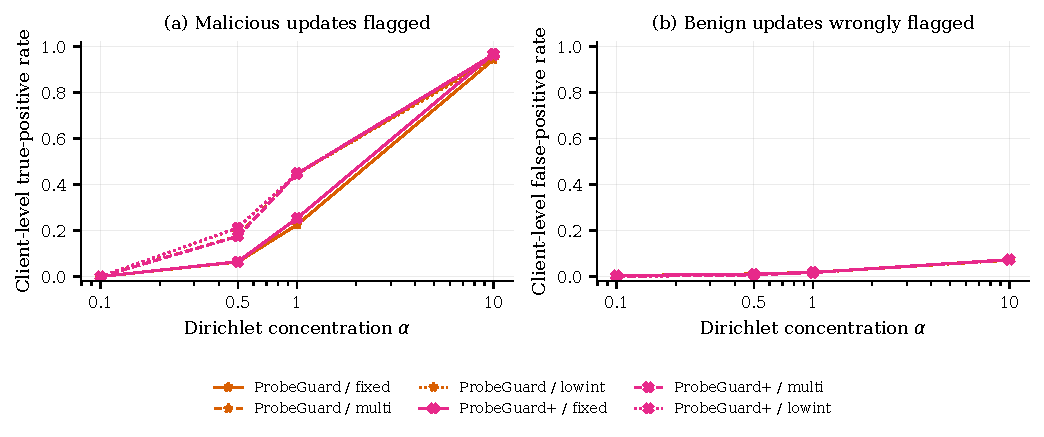
\includegraphics[width=0.64\textwidth]{fig_detect.pdf}
\caption{Client-level true-positive and false-positive rates of the MAD rule across heterogeneity levels.}\label{fig:detect}
\end{figure}
Detection under the MAD rule (Fig.~\ref{fig:detect}) mirrors the ASR pattern: TPR is 0.94 at $\alpha{=}10$ (FPR 0.07) but 0.23 at $\alpha{=}1$ and near zero at $\alpha\le0.5$. To determine whether the \emph{score} or the \emph{rule} is at fault, we logged scores along benign-only trajectories (19{,}200 client-round scores) and computed threshold-free AUROC (Fig.~\ref{fig:auroc}).
\begin{figure}[htbp]
\centering
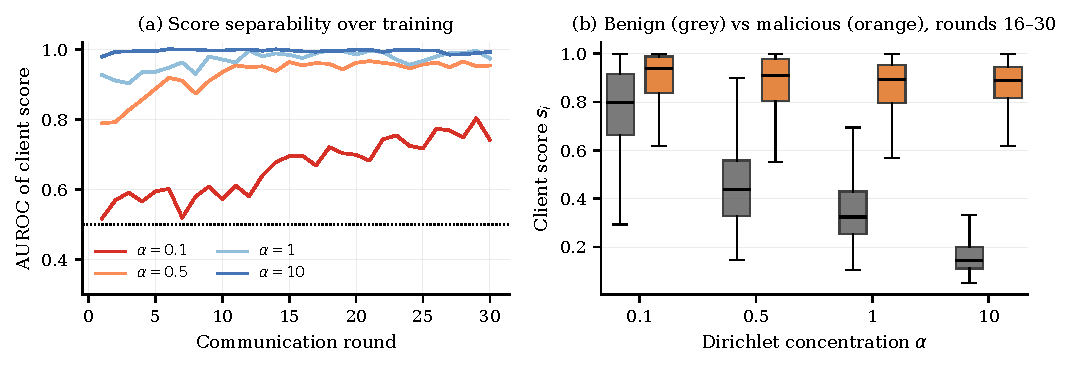
\includegraphics[width=0.64\textwidth]{fig_auroc.pdf}
\caption{(a) AUROC of the client score per round. (b) Benign and malicious score distributions in rounds 16--30.}\label{fig:auroc}
\end{figure}
Late-round (rounds 16--30) AUROC is $0.72\pm0.06$ ($\alpha{=}0.1$), $0.949\pm0.020$ (0.5), $0.978\pm0.012$ (1) and $0.993\pm0.008$ (10) (95\% CI over seeds). Early-round (rounds 1--5) AUROC is much lower for small $\alpha$ (0.57, 0.83, 0.92, 0.99), because the local backdoor has not yet formed. Hence at $\alpha\in\{0.5,1\}$ the representation is informative, while a fixed MAD threshold is a poor decision rule, and early misses let the global model acquire the backdoor, after which malicious updates deviate less. At $\alpha{=}0.1$ the score itself is only moderately informative. AUPRC (which accounts for the 20\% malicious base rate) tracks AUROC closely: $0.338, 0.823, 0.927, 0.964$ for $\alpha=0.1,0.5,1,10$ -- the score is not merely ranking well while being uninformative about actual malicious \emph{probability}.

\paragraph{Mechanism: measuring $\Delta_B$ directly.} Proposition~\ref{prop1} predicts that detection failure should track benign score spread. Fig.~\ref{fig:deltaB}a confirms heterogeneity drives this spread across nine $\alpha$ levels ($0.1$ to $10$): mean benign score standard deviation falls from $0.159$ to $0.118$, dropping sharply between $\alpha{=}0.5$ and $\alpha{=}1$. Fig.~\ref{fig:deltaB}b relates this directly to the MAD rule's TPR at each $\alpha$: $r=-0.81$ ($n=9$, $p=0.009$) -- with nine $\alpha$ levels this correlation is now statistically significant (an earlier four-point check gave the same direction but $p=0.18$), giving confirmatory rather than merely suggestive support for the mechanism.
\begin{figure}[htbp]
\centering
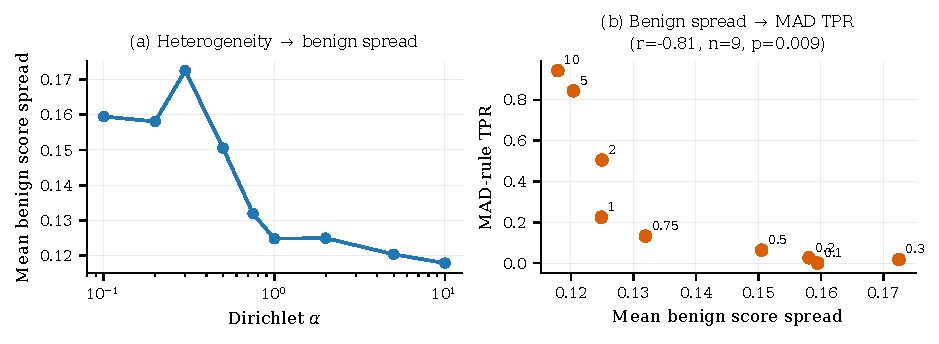
\includegraphics[width=0.64\textwidth]{fig_deltaB.pdf}
\caption{(a) Heterogeneity increases mean benign score spread (std.\ dev.\ of benign client scores, rounds 16--30). (b) That spread tracks the MAD rule's TPR across $\alpha$.}\label{fig:deltaB}
\end{figure}

\subsection{Score quality versus decision quality: a decision-rule sweep}\label{sec:killer}
The preceding results (AUROC/AUPRC above) show the score degrading only moderately as $\alpha$ falls to $0.5$--$1$, while the MAD rule's realised ASR degrades far more sharply -- Fig.~\ref{fig:killer} makes this divergence the paper's central figure. Panel (a) shows four decision rules applied to the identical score; panel (b) shows the ROC operating curves are far from the diagonal even at $\alpha=0.1$ (AUROC $0.72$), confirming some signal survives even where the MAD rule's realised ASR is no better than FedAvg's.
\begin{figure}[htbp]
\centering
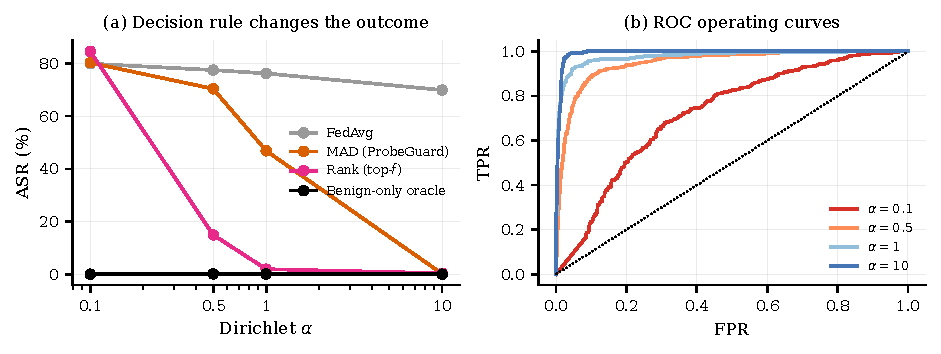
\includegraphics[width=0.68\textwidth]{fig_killer.pdf}
\caption{Score quality versus decision quality. (a) realised ASR under four decision rules applied to the identical score, across heterogeneity; (b) ROC operating curves, with the MAD rule's implicit operating point far from optimal at low $\alpha$.}\label{fig:killer}
\end{figure}
To test whether a \emph{better} threshold recovers the gap, Table~\ref{tab:decisionrules} compares six decision rules on the identical score: the MAD rule, three fixed percentile thresholds (90th/95th/97.5th), the rank-based rule (ProbeGuard-K, Section~\ref{sec:rankrule}), and an oracle threshold (uses ground-truth labels; an analysis ceiling, not a deployable rule). Percentile thresholds do \emph{not} fix the problem -- at $\alpha{=}0.1$ all three leave ASR within a few points of FedAvg, because a fixed percentile assumes a roughly constant malicious fraction and fails when the benign/malicious score gap itself closes. The rank-based rule is the only non-oracle rule that tracks the oracle-threshold ceiling closely for $\alpha\ge0.5$, diverging from it only at $\alpha{=}0.1$ (where Fig.~\ref{fig:deltaB} shows benign spread is largest). This localises the paper's failure mode precisely: \emph{not} absent signal, but a threshold family (fixed MAD, fixed percentile) that cannot adapt to how benign spread changes with heterogeneity; a rank-based rule that implicitly adapts to the current round's score distribution does much better, though still not perfectly at the most extreme heterogeneity tested.
\begin{table}[htbp]
\caption{Decision-rule sweep: ASR (\%), mean $\pm$ 95\% CI over 8 seeds, same score, fixed trigger, 20\% malicious.}\label{tab:decisionrules}
\centering\footnotesize
\setlength{\tabcolsep}{3pt}\begin{tabular}{@{}lcccc@{}}
\toprule
Decision rule & $\alpha{=}0.1$ & $\alpha{=}0.5$ & $\alpha{=}1$ & $\alpha{=}10$\\
\midrule
FedAvg & 79.9$\pm$13.3 & 77.4$\pm$5.5 & 76.2$\pm$5.7 & 69.9$\pm$3.4\\
MAD (ProbeGuard) & 80.2$\pm$13.4 & 70.3$\pm$6.7 & 46.8$\pm$21.4 & 0.3$\pm$0.2\\
90th pct. & 81.8$\pm$12.3 & 61.9$\pm$8.7 & 55.4$\pm$10.7 & 38.0$\pm$9.8\\
95th pct. & 81.0$\pm$12.6 & 71.6$\pm$6.7 & 68.4$\pm$7.7 & 57.7$\pm$6.4\\
97.5th pct. & 81.0$\pm$12.6 & 71.6$\pm$6.7 & 68.4$\pm$7.7 & 57.9$\pm$6.7\\
Rank (top-$f$) & 84.5$\pm$14.9 & 15.0$\pm$16.5 & 2.0$\pm$2.0 & 0.5$\pm$0.5\\
Oracle threshold & 0.1$\pm$0.1 & 0.2$\pm$0.2 & 0.2$\pm$0.3 & 0.1$\pm$0.1\\
Benign-only oracle & 0.1$\pm$0.1 & 0.2$\pm$0.2 & 0.2$\pm$0.3 & 0.1$\pm$0.1\\
\bottomrule
\end{tabular}
\end{table}

\subsection{A post-hoc rank-based rule on unseen seeds}\label{sec:rankrule}
\begin{table}[htbp]
\caption{Unseen seeds 20--27, 20\% malicious clients; ASR (\%), mean $\pm$ 95\% CI. ProbeGuard-K was designed after the analysis above.}\label{tab:fresh}
\centering\footnotesize
\setlength{\tabcolsep}{3.5pt}\begin{tabular}{@{}lcccc@{}}
\toprule
Defence & $\alpha{=}0.1$ & $\alpha{=}0.5$ & $\alpha{=}1$ & $\alpha{=}10$\\
\midrule
\multicolumn{5}{@{}l}{\emph{Fixed 2$\times$2 trigger: ASR (\%)}}\\
FedAvg & 86.3$\pm$7.4 & 72.5$\pm$10.5 & 74.9$\pm$6.0 & 69.7$\pm$10.9\\
Coord. median & 28.6$\pm$12.9 & 5.0$\pm$2.4 & 3.0$\pm$2.7 & 0.9$\pm$0.8\\
Multi-Krum & 89.3$\pm$6.3 & 70.0$\pm$22.4 & 10.9$\pm$13.3 & 15.4$\pm$16.9\\
FLTrust & 50.6$\pm$22.5 & 5.0$\pm$4.5 & 2.0$\pm$2.1 & 0.9$\pm$1.4\\
ProbeGuard (MAD rule) & 86.7$\pm$7.5 & 57.0$\pm$19.5 & 30.5$\pm$19.6 & 0.9$\pm$0.8\\
ProbeGuard-K (top-$f$ rule) & 89.1$\pm$7.8 & 4.8$\pm$3.2 & 6.3$\pm$8.0 & 1.0$\pm$0.9\\
Oracle (benign only) & 1.3$\pm$1.5 & 0.1$\pm$0.1 & 0.1$\pm$0.2 & 0.3$\pm$0.4\\
\midrule
\multicolumn{5}{@{}l}{\emph{Multi-location trigger: ASR (\%)}}\\
FedAvg & 36.9$\pm$11.7 & 24.5$\pm$7.9 & 23.8$\pm$8.9 & 16.9$\pm$3.1\\
Coord. median & 15.5$\pm$8.2 & 4.0$\pm$1.7 & 2.0$\pm$1.9 & 1.0$\pm$0.4\\
Multi-Krum & 46.8$\pm$15.4 & 12.8$\pm$8.4 & 1.8$\pm$3.1 & 2.1$\pm$2.0\\
FLTrust & 12.0$\pm$8.3 & 1.1$\pm$0.8 & 0.8$\pm$0.8 & 0.4$\pm$0.3\\
ProbeGuard (MAD rule) & 36.7$\pm$12.2 & 9.4$\pm$6.8 & 2.7$\pm$2.7 & 0.5$\pm$0.3\\
ProbeGuard-K (top-$f$ rule) & 27.3$\pm$12.0 & 1.0$\pm$0.5 & 1.4$\pm$2.3 & 0.6$\pm$0.3\\
Oracle (benign only) & 1.0$\pm$0.9 & 0.3$\pm$0.3 & 0.4$\pm$0.6 & 0.3$\pm$0.2\\
\bottomrule
\end{tabular}
\end{table}
Motivated by the AUROC analysis, ProbeGuard-K removes the $f$ highest-scoring clients each round. On unseen seeds (Table~\ref{tab:fresh}) it reaches 4.8\% and 6.3\% ASR at $\alpha{=}0.5$ and $1$ (fixed trigger), versus 57.0\% and 30.5\% for the MAD rule; differences from coordinate median and FLTrust at these levels are not significant with 8 seeds (paired $p\ge0.38$), which does not establish equivalence. At $\alpha{=}0.1$ it fails (89.1\%; TPR 0.07, FPR 0.23). It requires knowing $f$, an assumption shared with Multi-Krum; Section~\ref{sec:sensitivity} below tests misspecified $f$ directly.

\subsection{Malicious fraction, system sensitivity, and cost}\label{sec:sensitivity}
\begin{figure}[htbp]
\centering
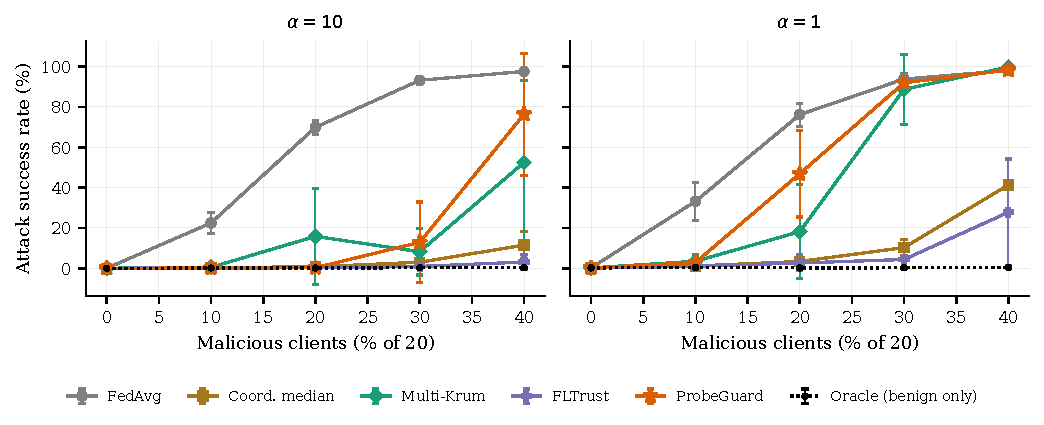
\includegraphics[width=0.6\textwidth]{fig_msweep.pdf}
\caption{ASR versus malicious fraction (fixed trigger).}\label{fig:msweep}
\end{figure}
Fig.~\ref{fig:msweep}: ProbeGuard's MAD rule holds to 20\% malicious at $\alpha{=}10$ (0.3\%), degrades at 30\% (12.9\%), fails at 40\% (76.4\%) -- $m<n/2$ alone does not guarantee practical robustness; the thresholded rule breaks well before the median-containment condition itself does. FLTrust degrades more gracefully (3.1\% at 40\%). Clean accuracy with no attackers is close to FedAvg throughout (89.7\% vs.\ 90.1\% at $\alpha{=}10$).

\paragraph{Scoring-rule ablation.} Three alternative scoring functions (own no-patch baseline, spatial localisation, bias-matched neighbours) were tested against the median reference; none improved on it at $\alpha{=}10$ (full table in supplementary material) -- a negative result that does not change our conclusions.

\paragraph{Root-set size, probe-bank size, and overhead.} ASR is insensitive to root-set size above 50 images and probe-bank density above 9 probes ($\alpha{=}1$; the 49-probe, 100-image default is not tightly required), but overhead is substantial: ProbeGuard's MAD/rank rules cost $4$--$5\times$ FedAvg's wall-clock time versus $<35\%$ for geometry-based baselines (full ablation in supplementary material).

\paragraph{Unknown $f$ (full table in supplementary material).} ProbeGuard-K/Multi-Krum both assume $f$ known; testing true $m{=}4$ (20\%) against assumed $f\in\{1,\dots,8\}$: \emph{under}-estimating is damaging for both (ASR 55--67\% at $f{=}1$), \emph{over}-estimating is safe for both (ASR $\le1\%$ at $f\ge5$) -- a deployer unsure of $m$ should round up. ProbeGuard-K's advantage is concentrated at correct/over-specified $f$ (0\% vs.\ 16--18\% at true $f{=}4$); under severe under-specification the two converge.

\paragraph{Attack trajectory and interpretability (details in supplementary material).} The same pattern persists across training, not just at round 30: at $\alpha{=}1$, mean 30-round ASR is 71.1\% for the MAD rule versus 72.4\% for FedAvg, while ProbeGuard-K reaches 10.1\% -- the MAD rule's failure is not a late-round convergence artefact. The spatial probe response also localises the implanted trigger (peak flip rate 0.98 for malicious clients vs.\ 0.38 for benign), supporting the score's interpretability beyond a scalar number.

\section{Adaptive attacker}\label{sec:adaptive}
Every result so far assumes a non-adaptive attacker (threat model, Section~\ref{sec4}). We relax this: malicious clients now know ProbeGuard is deployed, the exact probe bank, the scoring rule, and the current global model.

\subsection{A probe-aware adaptive attack}
Each malicious client's local loss becomes $L_{\text{backdoor}}+\beta\cdot L_{\text{stealth}}$: the standard backdoor cross-entropy on the poisoned batch, plus a cross-entropy term (weight $\beta$) pushing predictions on \emph{clean} images patched at a random \emph{non-trigger} probe-bank cell back toward their true label. This penalises exactly the bank-wide flip-rate elevation driving the ProbeGuard score, leaving the true trigger cell untouched (suppressing it would weaken the backdoor itself -- it is one bank cell by construction, Section~\ref{sec4}). We sweep $\beta\in\{0,0.1,0.25,0.5\}$ at $\alpha\in\{1,10\}$, fixed trigger, 20\% malicious, 5 seeds, against FedAvg, Multi-Krum, ProbeGuard (MAD), and ProbeGuard-K.

\subsection{Results}
\begin{figure}[htbp]
\centering
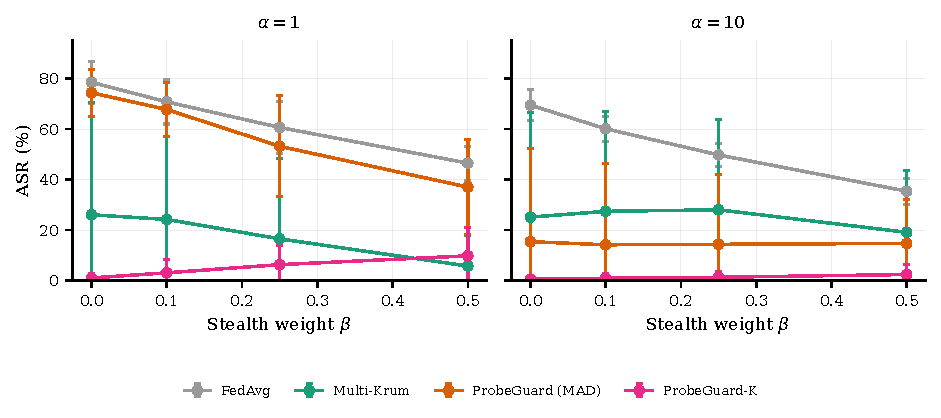
\includegraphics[width=0.62\textwidth]{fig_adaptive.pdf}
\caption{ASR versus attacker stealth weight $\beta$, by defence and heterogeneity.}\label{fig:adaptive}
\end{figure}
\begin{table}[htbp]
\caption{Non-adaptive vs.\ adaptive ($\beta{=}0.5$) attacker; mean $\pm$ 95\% CI over 5 seeds. TPR is the defence's client-flagging rate where applicable.}\label{tab:adaptive}
\centering\footnotesize\begin{tabular}{@{}llcccc@{}}
\toprule
Defence & Attack & $\alpha=1$ ASR (\%) & $\alpha=1$ TPR & $\alpha=10$ ASR (\%) & $\alpha=10$ TPR\\
\midrule
FedAvg & non-adaptive & 78.5$\pm$8.2 & -- & 69.5$\pm$6.2 & --\\
FedAvg & adaptive ($\beta{=}0.5$) & 46.5$\pm$6.8 & -- & 35.4$\pm$5.2 & --\\
\addlinespace
Multi-Krum & non-adaptive & 26.1$\pm$44.3 & -- & 25.1$\pm$41.3 & --\\
Multi-Krum & adaptive ($\beta{=}0.5$) & 5.8$\pm$11.9 & -- & 19.1$\pm$24.6 & --\\
\addlinespace
ProbeGuard (MAD) & non-adaptive & 74.3$\pm$9.4 & 0.03 & 15.4$\pm$37.0 & 0.57\\
ProbeGuard (MAD) & adaptive ($\beta{=}0.5$) & 37.0$\pm$18.8 & 0.07 & 14.7$\pm$17.4 & 0.38\\
\addlinespace
ProbeGuard-K & non-adaptive & 1.0$\pm$1.6 & 0.86 & 0.6$\pm$0.9 & 0.94\\
ProbeGuard-K & adaptive ($\beta{=}0.5$) & 9.8$\pm$11.3 & 0.62 & 2.4$\pm$3.9 & 0.79\\
\addlinespace
\bottomrule
\end{tabular}
\end{table}
Fig.~\ref{fig:adaptive}: increasing $\beta$ \emph{lowers the attacker's own achievable ASR} against every defence, including undefended FedAvg (69.5\%$\to$35.4\% at $\alpha{=}10$) -- stealth is not free here. Table~\ref{tab:adaptive} gives the attacker's strongest tested setting ($\beta{=}0.5$). ProbeGuard-K remains most robust at both heterogeneity levels: at $\alpha{=}10$ its adaptive ASR (2.4\%) stays far below FedAvg's non-adaptive ceiling (69.5\%), rising only 1.8\,pp over its own non-adaptive ASR; at $\alpha{=}1$ the attacker does better against it (9.8\% vs.\ 1.0\%, TPR 0.86$\to$0.62) -- consistent with heterogeneity being this defence family's weak point. The MAD rule, already weak, is not made meaningfully worse by adaptation. A more targeted variant (re-attacking the single highest-flip-rate non-trigger cell each round, instead of a random cell) did not meaningfully increase ASR against ProbeGuard-K ($10.2\%$ vs.\ $9.8\%$ at $\alpha{=}1,\beta{=}0.5$). This remains two strategies among many; a stronger optimiser could not be ruled out.

\section{CNN-scale stress test on CIFAR-10}\label{sec:cnn}
The preceding sections use an 8$\times$8-digit MLP -- a real limitation, discussed further in Section~\ref{sec7} below. To check whether the central finding survives at a more realistic scale, we ran a smaller, compute-constrained stress test on CIFAR-10 with a 3-layer CNN (189k parameters), on a single CPU laptop (no GPU). Because of the resulting compute budget, this validation covers 3 seeds rather than 8, two values of $\alpha$ rather than four, and only the fixed trigger; it is a check on the main finding, not a replacement for Sections~\ref{sec6}--\ref{sec:adaptive}. All CNN code, raw outputs, and the commands used are included in the supplementary material's \texttt{cnn/} directory.

\paragraph{Setup.} 20 clients, 20\% malicious, Dirichlet splits over CIFAR-10's training set, a 200-image server root set, local SGD (1 epoch/round, batch 32). We report two independent settings at $\alpha{=}10$: (i) the full $\sim$50{,}000-image training pool at 15 rounds, and (ii) a 25{,}000-image subset at 30 rounds, run to check whether more communication rounds change the picture. A third, 10{,}000-image configuration is excluded: the benign-only oracle itself reached only $\sim$10\% accuracy there (chance level), making ASR uninterpretable. Clean accuracy here is well below full-training CIFAR-10 (limited rounds/data, same budget for every defence), so we report ASR \emph{relative to the benign-only oracle under identical conditions} (``lift'' $=$ ASR$_{\text{defence}}-$ASR$_{\text{oracle}}$, same seed) as the primary comparison.

\begin{table}[htbp]
\caption{CIFAR-10, CNN, 50k images / 15 rounds, 20\% malicious, fixed trigger. Mean $\pm$ 95\% CI over 3 seeds (wide intervals reflect $n=3$).}\label{tab:cnn-main}
\centering\footnotesize
\setlength{\tabcolsep}{4pt}\begin{tabular}{@{}lcccc@{}}
\toprule
Defence & \multicolumn{2}{c}{$\alpha=1$} & \multicolumn{2}{c}{$\alpha=10$}\\
 & ASR (\%) & Acc (\%) & ASR (\%) & Acc (\%)\\
\midrule
FedAvg & 73.9$\pm$20.2 & 28.5$\pm$3.0 & 60.4$\pm$32.6 & 29.7$\pm$1.5\\
Coord. median & 36.5$\pm$15.5 & 22.5$\pm$5.7 & 20.3$\pm$9.7 & 28.0$\pm$2.4\\
Multi-Krum & 14.9$\pm$10.8 & 29.0$\pm$4.6 & 12.6$\pm$8.5 & 30.0$\pm$3.2\\
FLTrust & 99.4$\pm$1.3 & 10.7$\pm$2.2 & 66.6$\pm$143.2 & 10.5$\pm$2.1\\
ProbeGuard (MAD) & 74.2$\pm$43.3 & 30.0$\pm$3.7 & 41.6$\pm$56.6 & 30.3$\pm$1.4\\
ProbeGuard-K & 40.2$\pm$98.2 & 30.2$\pm$3.8 & 14.7$\pm$9.4 & 30.2$\pm$3.0\\
Oracle (benign only) & 13.3$\pm$9.1 & 29.7$\pm$5.2 & 12.4$\pm$8.5 & 30.0$\pm$3.2\\
\bottomrule
\end{tabular}
\end{table}

\begin{figure}[htbp]
\centering
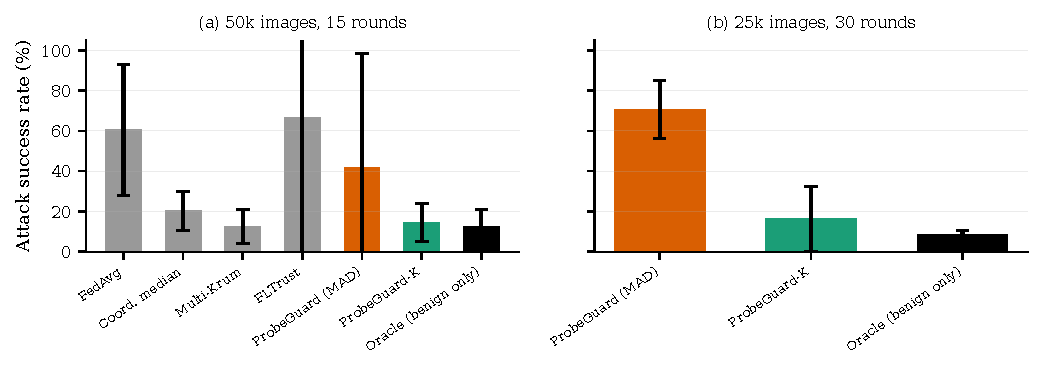
\includegraphics[width=0.65\textwidth]{fig_cnn_alpha10.pdf}
\caption{ASR at $\alpha{=}10$ in two independent CNN settings: (a) the main 50k/15-round run (all baselines); (b) a 25k/30-round re-run isolating ProbeGuard, ProbeGuard-K and the oracle. Error bars: 95\% CI over 3 seeds.}\label{fig:cnn-bar}
\end{figure}

\begin{table}[htbp]
\caption{Oracle-adjusted lift (ASR$_{\text{defence}}-$ASR$_{\text{oracle}}$, same seed) for the two ProbeGuard variants, at $\alpha{=}10$, in both independent CNN settings.}\label{tab:cnn-lift}
\centering\footnotesize\begin{tabular}{@{}lccc@{}}
\toprule
Setting & Seed & ProbeGuard lift (pp) & ProbeGuard-K lift (pp)\\
\midrule
50k images, 15 rounds & 0 & +42.7 & +0.2\\
50k images, 15 rounds & 1 & +39.4 & +6.5\\
50k images, 15 rounds & 2 & +5.4 & -0.1\\
\addlinespace
25k images, 30 rounds & 0 & +67.5 & +11.0\\
25k images, 30 rounds & 1 & +55.8 & -0.2\\
25k images, 30 rounds & 2 & +63.8 & +12.7\\
\addlinespace
\bottomrule
\end{tabular}
\end{table}

\paragraph{Finding 1: the threshold-vs-score gap widens, not narrows, on CNNs.} At $\alpha{=}10$ -- where the digits-scale MAD rule was near-perfect (0.3\% ASR) -- it instead performs \emph{worse than FedAvg} here (41.6\% vs.\ 60.4\%; Table~\ref{tab:cnn-main}). Its lift over the oracle is $+5$ to $+68$\,pp across both independent settings (Table~\ref{tab:cnn-lift}) -- substantially worse than doing nothing, consistently. This diverges from, rather than replicates, the digits-scale result.

\paragraph{Finding 2: the rank-based rule is far more robust, in both settings.} ProbeGuard-K's lift is near zero in 4 of 6 seed/setting combinations and modest in the rest ($+6.5$ to $+12.7$\,pp), close to Multi-Krum's level rather than FedAvg's. This held across both data-volume and round-count changes tested, evidence against a single-run artefact, and is consistent with Section~\ref{sec6}: the score may separate clients reasonably well, but a fixed MAD threshold is the wrong rule for it -- more so on CNNs than the MLP (AUROC diagnostic not run at CNN scale, compute cost).

\paragraph{Finding 3 (unresolved): FLTrust underperforms FedAvg at CNN scale.} FLTrust reaches 99.4\%/66.6\% ASR at $\alpha{=}1,10$, worse than FedAvg, with accuracy pinned near chance ($\sim$10--11\%) across every seed and both learning rates tried, ruling out learning rate alone. Likely mechanism, \emph{not confirmed}: a single-epoch, 200-image root-gradient estimate may be too noisy against a 189k-parameter CNN -- FLTrust stays robust on the digits MLP even with 10 root images, ruling out small root size alone. \textbf{Flagged as unresolved.}

\paragraph{Scope.} Three seeds, wide CIs, no paired tests. One trigger, two heterogeneity levels; no CNN-scale ablations. More rounds (25k/30) did not fix the MAD rule (partial data-volume confound). Read this as evidence the digits-scale finding's \emph{direction may not generalise safely} to CNNs.


\section{Discussion and limitations}\label{sec7}
The main lesson is methodological: a behavioural score can be highly discriminative (Fig.~\ref{fig:killer}a) while every \emph{fixed} threshold tested -- MAD, three percentile levels -- still fails under heterogeneity (Table~\ref{tab:decisionrules}); only a rank-based rule that adapts to the current score distribution closes most of the gap to an oracle threshold, and remains comparatively robust under one tested adaptive attack (Section~\ref{sec:adaptive}). Rules and representations should be evaluated separately (threshold-free AUROC/AUPRC alongside realised ASR) rather than reporting ASR alone, which conflates the two. Limitations, listed without softening: (1) scale -- 8$\times$8 digits, a small MLP, 20 clients; the CNN stress test (Section~\ref{sec:cnn}, 3 seeds, 2 settings) suggests the failure mode does not shrink at larger scale but is not a full replication. (2) the adaptive attack (Section~\ref{sec:adaptive}) is one specific, moderately-tuned strategy, not an exhaustive or adversarially-optimal search; stronger attacks remain possible. (3) ProbeGuard/FLTrust assume a small clean root set; ProbeGuard-K/Multi-Krum additionally assume known $f$ -- now tested under misspecification (Section~\ref{sec6}), finding over-estimation safe and under-estimation damaging for both. (4) baselines are simplified re-implementations. (5) $k,\delta$ were tuned at $\alpha{=}1$, where the MAD rule is weak; percentile/rank rules used no equivalent tuning. (6) ProbeGuard-K was designed after inspecting seeds 0--7, evaluated on unseen seeds 20--27 for its headline numbers; the decision-rule sweep reuses seeds 0--7 and is exploratory for that comparison. (7) eight seeds (five for the adaptive-attack grid) limit power; non-significance is reported as non-significance, not equivalence. (8) the $\Delta_B$--TPR correlation ($n=4$) is supporting, not confirmatory, evidence. (9) leave-one-trigger-family-out generalisation and formal statistical models beyond paired Wilcoxon/Holm (mixed-effects, bootstrap, equivalence testing) were cut for length rather than run superficially.

\section{Conclusion}\label{sec8}
Behavioural trigger probing is a strong detector near-IID and yields interpretable trigger localisation, but with a fixed threshold it does not survive strong heterogeneity, even though its scores remain discriminative. A rank-based decision rule recovers most of this gap and remains comparably robust under a CNN stress test (Section~\ref{sec:cnn}, where the gap instead widens) and one adaptive attacker (Section~\ref{sec:adaptive}). This is a reason for cautious optimism about the decision-rule fix specifically, and continued caution about fixed-threshold behavioural probing generally, in realistic deployments. Future work should test CNN models on larger benchmarks with more seeds, run the AUROC and ablation diagnostics at CNN scale, resolve the open FLTrust observation (Section~\ref{sec:cnn}), test stronger/optimiser-based adaptive attacks and unknown $f$, and study heterogeneity-aware thresholds or soft weighting.

\backmatter
\bmhead{Data and code availability}
The dataset is bundled with scikit-learn. All experiment code (NumPy) and raw per-run results accompany this manuscript and will be released publicly upon acceptance.

\section*{Declarations}
\textbf{Competing interests.} The author is the founder of FedGuard Private Limited, a company working on federated-learning security. \textbf{Funding.} None declared.

{\fontsize{9.3pt}{11pt}\selectfont\bibliography{refs}}

\end{document}
